\documentclass[12pt]{article}

\usepackage{sbc-template}
\usepackage{graphicx,url}
\usepackage[brazil]{babel}
\usepackage[utf8]{inputenc}
\usepackage{relsize}
\usepackage{amsmath}

%\renewcommand{\inst}[1]{} % esconde o numero da instituição

\sloppy

\title{
  Desenvolvimento de uma Ferramenta Integrada ao Google Earth Engine para
  a Análise de Ambientes Costeiros
}

\author{
  Fernando Concatto\inst{1}, Luis Pedro Almeida\inst{3}, Rodrigo Lyra\inst{1},\\
  Arthur A. Machado \inst{2}, Rudimar L. S. Dazzi\inst{1}, Antonio H. F. Klein \inst{2}
}

\address{
  Universidade do Vale do Itajaí (UNIVALI)
\nextinstitute
  Universidade Federal de Santa Catarina (UFSC)
\nextinstitute
  Centre National d'Études Spatiales (CNES)
\email{fernandoconcatto@gmail.com, melolp@gmail.com}
}

\begin{document}

\maketitle

\begin{abstract}
  Coastal zones are among the regions most impacted by climate change; understanding their evolution along the years is essential to handle the damage they suffered. This work proposes a tool to analyze coastal zones of the entire planet through the usage of Google Earth Engine, a platform for performing multispectral image processing and data visualization in the cloud.
\end{abstract}

\section{Introdução} \label{sec:intro}

Regiões costeiras do planeta Terra estão intensamente ameaçadas por mudanças climáticas, causadas tanto por fatores naturais quanto antrópicos, como a rápida urbanização e industrialização \cite{Bird1985}. As mudanças mais significativas observadas nestas regiões incluem a retração de linhas de costa e o desmatamento de áreas de vegetação para ocupação humana e atividades agrícolas \cite{Ferreira2006}. Neste contexto, o mapeamento e classificação da ocupação do solo em zonas costeiras torna-se uma tarefa crucial para a adequada gestão e tomada de decisões mitigatórias. Tais atividades podem ser realizadas por meio do processamento de imagens multiespectrais e outros dados coletados por meio de satélites \cite{Bansal2017,Othman2014}.

Ao longo dos últimos anos, a Google vem desenvolvendo uma plataforma baseada em \textit{cloud computing} chamada Google Earth Engine (GEE), a qual tem por objetivo habilitar a aplicação de algoritmos de descoberta de conhecimento e a visualização de dados em escala planetária, utilizando bases de dados de diversas missões de satélite e uma interface de desenvolvimento integrada  \cite{Gorelick2017}.

Este trabalho visa apresentar o desenvolvimento de uma ferramenta que faz uso das capacidades do GEE e sua API para permitir a análise das dinâmicas de diferentes características de regiões costeiras, tendo como público-alvo tanto pesquisadores quanto gestores e usuários com conhecimentos limitados de programação.

\section{Solução Proposta} \label{sec:psolution}

A ferramenta proposta neste trabalho busca equilibrar três fatores distintos: \textit{(i)} funcionalidades, oferecendo meios para a realização de diversos tipos de análises quanto à evolução de feições costeiras; \textit{(ii)} desempenho, sendo capaz de processar grandes massas de dados rapidamente, com a assistência do GEE; e \textit{(iii)} complexidade, podendo ser utilizada sem grandes dificuldades por usuários desprovidos de conhecimento profundo em programação. Para tanto, se fez necessária a realização de uma desassociação da interface de utilizador oferecida pela Google em direção a uma aplicação construída separadamente, mas capaz de se comunicar com a plataforma GEE para efetuar a obtenção e o processamento de dados. Este desacoplamento permite a personalização completa do sistema, habilitando o ajuste fino dos fatores estabelecidos anteriormente.

A arquitetura geral do sistema é apresentada na Figura \ref{fig:arch}. O usuário interage diretamente com uma aplicação Web em seu navegador, através da qual será possível requisitar análises de qualquer região do planeta e visualizar resultados em formato de gráficos, tabelas e em mapas. A aplicação, por sua vez, constrói a sequência de operações necessárias para satisfazer a demanda do usuário e delega sua execução para o \textit{cluster} de processamento do GEE através de requisições HTTP assíncronas. Ao concluir os procedimentos, a API retorna os resultados para a aplicação em formato GeoJSON, e a mesma fica encarregada de apresentar graficamente tais dados para o usuário.

\begin{figure}[ht]
  \vspace{0.1cm}
  \centering
  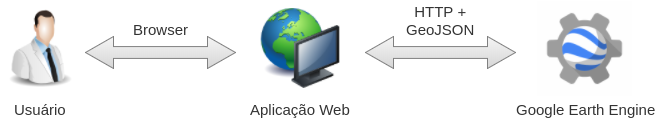
\includegraphics[width=.64\textwidth]{cassie.png}
  \vspace{0.05cm}
  \caption{Arquitetura da ferramenta proposta}
  \label{fig:arch}
\end{figure}

\section{Considerações Finais} \label{sec:discussion}

A utilização das capacidades de processamento em nuvem do Google Earth Engine habilita a análise de imagens multiespectrais de alta resolução sem a necessidade de investimentos financeiros em computadores de alto desempenho, bastando apenas um dispositivo conectado à Internet. Testes preliminares indicam que é possível realizar operações fundamentais para o contexto desta proposta, como aplicação de filtros, extração de histogramas, vetorização e cálculo de índices de água e vegetação sobre extensos conjuntos de imagens (1984--2017) através de chamadas ao Google Earth Engine em tempo hábil e apresentar tais dados graficamente por meio da API do Google Maps, sendo possível visualizar e manipular tanto informações geométricas quando matriciais (\textit{rasters}).

\bibliographystyle{sbc}
\bibliography{sbc-template}

\end{document}
